\documentclass[14pt]{extbook}
\usepackage{multicol, enumerate, enumitem, hyperref, color, soul, setspace, parskip, fancyhdr} %General Packages
\usepackage{amssymb, amsthm, amsmath, bbm, latexsym, units, mathtools} %Math Packages
\everymath{\displaystyle} %All math in Display Style
% Packages with additional options
\usepackage[headsep=0.5cm,headheight=12pt, left=1 in,right= 1 in,top= 1 in,bottom= 1 in]{geometry}
\usepackage[usenames,dvipsnames]{xcolor}
\usepackage{dashrule}  % Package to use the command below to create lines between items
\newcommand{\litem}[1]{\item#1\hspace*{-1cm}\rule{\textwidth}{0.4pt}}
\pagestyle{fancy}
\lhead{Progress Quiz 5}
\chead{}
\rhead{Version A}
\lfoot{9912-2038}
\cfoot{}
\rfoot{Spring 2021}
\begin{document}

\begin{enumerate}
\litem{
Solve the linear equation below. Then, choose the interval that contains the solution.\[ \frac{3x + 8}{5} - \frac{-5x + 5}{8} = \frac{4x -7}{6} \]\begin{enumerate}[label=\Alph*.]
\item \( x \in [-4.3, -3.7] \)
\item \( x \in [-19.7, -15.6] \)
\item \( x \in [-2.1, 1] \)
\item \( x \in [-6.3, -5.2] \)
\item \( \text{There are no real solutions.} \)

\end{enumerate} }
\litem{
Write the equation of the line in the graph below in Standard form $Ax+By=C$. Then, choose the intervals that contain $A, B, \text{ and } C$.
\begin{center}
    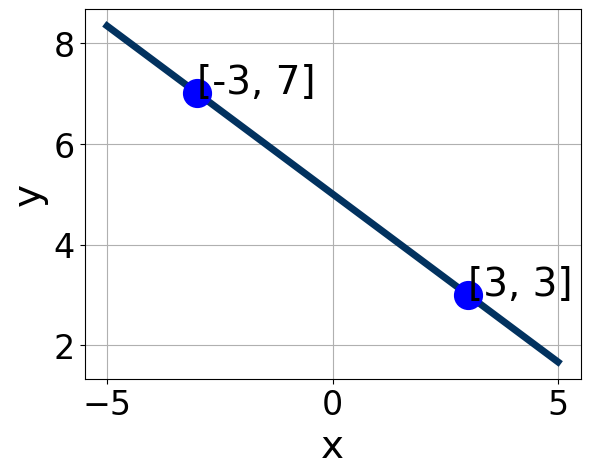
\includegraphics[width=0.5\textwidth]{../Figures/linearGraphToStandardA.png}
\end{center}
\begin{enumerate}[label=\Alph*.]
\item \( A \in [0.94, 3.08], \hspace{3mm} B \in [1.74, 3.82], \text{ and } \hspace{3mm} C \in [14, 17] \)
\item \( A \in [-2.12, 0.01], \hspace{3mm} B \in [-3.47, -2.28], \text{ and } \hspace{3mm} C \in [-17, -11] \)
\item \( A \in [0.94, 3.08], \hspace{3mm} B \in [-3.47, -2.28], \text{ and } \hspace{3mm} C \in [-17, -11] \)
\item \( A \in [-0.55, 1.4], \hspace{3mm} B \in [-1.53, -0.25], \text{ and } \hspace{3mm} C \in [-5, 0] \)
\item \( A \in [-0.55, 1.4], \hspace{3mm} B \in [0.51, 1.44], \text{ and } \hspace{3mm} C \in [1, 7] \)

\end{enumerate} }
\litem{
Solve the equation below. Then, choose the interval that contains the solution.\[ -15(-10x + 11) = -5(-9x + 13) \]\begin{enumerate}[label=\Alph*.]
\item \( x \in [0.68, 1.1] \)
\item \( x \in [1, 1.55] \)
\item \( x \in [1.64, 2.34] \)
\item \( x \in [-2.42, -1.74] \)
\item \( \text{There are no real solutions.} \)

\end{enumerate} }
\litem{
First, find the equation of the line containing the two points below. Then, write the equation as $ y=mx+b $ and choose the intervals that contain $m$ and $b$.\[ (-10, 4) \text{ and } (4, -11) \]\begin{enumerate}[label=\Alph*.]
\item \( m \in [-4.5, 0.4] \hspace*{3mm} b \in [-7.28, -6.11] \)
\item \( m \in [-4.5, 0.4] \hspace*{3mm} b \in [6.37, 7.69] \)
\item \( m \in [-4.5, 0.4] \hspace*{3mm} b \in [-15.23, -14.5] \)
\item \( m \in [-4.5, 0.4] \hspace*{3mm} b \in [13.91, 14.41] \)
\item \( m \in [-1, 2.8] \hspace*{3mm} b \in [-15.63, -15.07] \)

\end{enumerate} }
\litem{
First, find the equation of the line containing the two points below. Then, write the equation as $ y=mx+b $ and choose the intervals that contain $m$ and $b$.\[ (5, 5) \text{ and } (-10, 7) \]\begin{enumerate}[label=\Alph*.]
\item \( m \in [-0.77, -0.06] \hspace*{3mm} b \in [13.8, 18] \)
\item \( m \in [-0.77, -0.06] \hspace*{3mm} b \in [-1.3, 1.6] \)
\item \( m \in [-0.77, -0.06] \hspace*{3mm} b \in [3.8, 7.3] \)
\item \( m \in [-0.77, -0.06] \hspace*{3mm} b \in [-9.4, -5] \)
\item \( m \in [0.01, 0.77] \hspace*{3mm} b \in [8.1, 9.1] \)

\end{enumerate} }
\litem{
Write the equation of the line in the graph below in Standard form $Ax+By=C$. Then, choose the intervals that contain $A, B, \text{ and } C$.
\begin{center}
    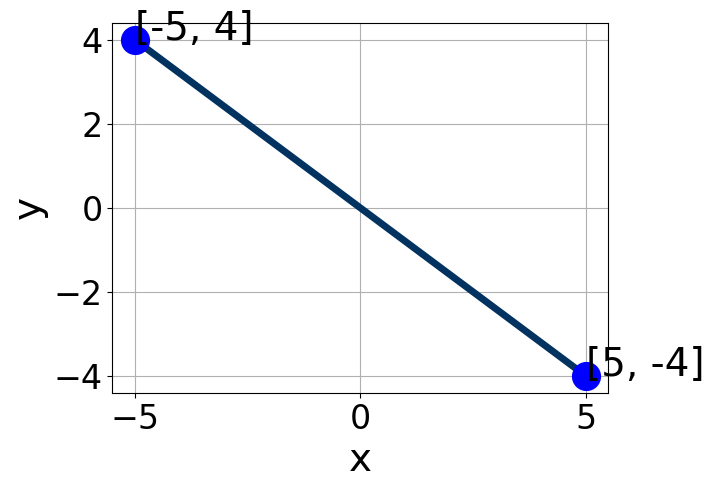
\includegraphics[width=0.5\textwidth]{../Figures/linearGraphToStandardCopyA.png}
\end{center}
\begin{enumerate}[label=\Alph*.]
\item \( A \in [-8, -3], \hspace{3mm} B \in [-6.1, -4.2], \text{ and } \hspace{3mm} C \in [-3, 5] \)
\item \( A \in [0.8, 2.8], \hspace{3mm} B \in [0.6, 2.4], \text{ and } \hspace{3mm} C \in [-3, 5] \)
\item \( A \in [3, 6], \hspace{3mm} B \in [3.3, 5.5], \text{ and } \hspace{3mm} C \in [-3, 5] \)
\item \( A \in [3, 6], \hspace{3mm} B \in [-6.1, -4.2], \text{ and } \hspace{3mm} C \in [-3, 5] \)
\item \( A \in [0.8, 2.8], \hspace{3mm} B \in [-1.4, -0.2], \text{ and } \hspace{3mm} C \in [-3, 5] \)

\end{enumerate} }
\litem{
Solve the equation below. Then, choose the interval that contains the solution.\[ -5(3x + 7) = -15(2x -8) \]\begin{enumerate}[label=\Alph*.]
\item \( x \in [-2.11, 2.89] \)
\item \( x \in [10.33, 12.33] \)
\item \( x \in [-9.67, -4.67] \)
\item \( x \in [3.67, 6.67] \)
\item \( \text{There are no real solutions.} \)

\end{enumerate} }
\litem{
Find the equation of the line described below. Write the linear equation as $ y=mx+b $ and choose the intervals that contain $m$ and $b$.\[ \text{Parallel to } 5 x + 8 y = 12 \text{ and passing through the point } (2, 6). \]\begin{enumerate}[label=\Alph*.]
\item \( m \in [-1.71, -1.51] \hspace*{3mm} b \in [6.69, 7.41] \)
\item \( m \in [0.29, 0.95] \hspace*{3mm} b \in [4.3, 5.37] \)
\item \( m \in [-0.99, -0.57] \hspace*{3mm} b \in [-8.27, -6.86] \)
\item \( m \in [-0.99, -0.57] \hspace*{3mm} b \in [6.69, 7.41] \)
\item \( m \in [-0.99, -0.57] \hspace*{3mm} b \in [2.81, 4.44] \)

\end{enumerate} }
\litem{
Solve the linear equation below. Then, choose the interval that contains the solution.\[ \frac{-3x + 6}{7} - \frac{3x + 8}{5} = \frac{-7x + 8}{8} \]\begin{enumerate}[label=\Alph*.]
\item \( x \in [1.74, 2.74] \)
\item \( x \in [-14.35, -9.35] \)
\item \( x \in [-66.12, -64.12] \)
\item \( x \in [8.49, 11.49] \)
\item \( \text{There are no real solutions.} \)

\end{enumerate} }
\litem{
Find the equation of the line described below. Write the linear equation as $ y=mx+b $ and choose the intervals that contain $m$ and $b$.\[ \text{Perpendicular to } 8 x - 5 y = 6 \text{ and passing through the point } (9, 10). \]\begin{enumerate}[label=\Alph*.]
\item \( m \in [-2.12, -1] \hspace*{3mm} b \in [14.62, 17.62] \)
\item \( m \in [-0.82, -0.62] \hspace*{3mm} b \in [14.62, 17.62] \)
\item \( m \in [-0.82, -0.62] \hspace*{3mm} b \in [-17.62, -13.62] \)
\item \( m \in [-0.82, -0.62] \hspace*{3mm} b \in [-1, 2] \)
\item \( m \in [0.6, 0.91] \hspace*{3mm} b \in [2.38, 12.38] \)

\end{enumerate} }
\end{enumerate}

\end{document}